\documentclass[12pt]{beamer}
\usepackage[T2A]{fontenc} 
\usepackage[utf8]{inputenc} 
\usepackage{algorithm}
\usepackage{algorithmic}
\usepackage[english, ukrainian]{babel} 
\mode<presentation>{
	\usetheme{CambridgeUS}
    \setbeamercovered{transparent}
}
%% preamble
\title{Ієрархічні матриці у методі граничних елементів}
\author{Солук Олена}
\date[ 2017]
{\large{Львівський національний університет імені І.Франка}}
\begin{document}
\begin{frame}
	\titlepage
\end{frame}
%% normal frame
\begin{frame}{Зміст}
\begin{block}{}
	1. Кластерне дерево i блочне кластерне дерево.\\
	2. Умова допустимості.\\
	3. Означення $\mathcal{H}$-матриці.\\
	4. Модельна задача BEM.\\
	5. Побудова $\mathcal{H}$-матриці(n-вимірний простір).\\
	6. Задача Діріхле для рівняння Лапласа.
\end{block}	
\end{frame}

\begin{frame}
\frametitle{Кластерне дерево}
	\begin{block}{Означення}
		Дерево $\mathbb{T}_{I}$ називається кластерне дерево над множиною індексів $I$ з $root(\mathbb{T}_{I})=I$, якщо наступні умови виконуються:
			\begin{enumerate}
				\item[-] $I \in V$ є коренем $\mathbb{T}_{I}$ i $\forall v \in V,v\not=\O \Rightarrow v\subseteq I$.
				\item[-] Якщо $v\in V$ не є листком ($S(v)\not=\O$), то він рівний об'єднанню своїх синів, тобто $v=\bigcup_{w\in S(v)}w$.
			\end{enumerate}
	\end{block}
\end{frame}

\begin{frame}
\frametitle{Блочне кластерне дерево}
	\begin{block}{Означення}
	Нехай $\mathbb{T}_{I}$ і $\mathbb{T}_{J}$ - кластерні дерева над множинами індексів $I$ та $J$ відповідно. Кластерне дерево $\mathbb{T}_{I\times J}=\mathbb{T}_{\mathbb{T}_{I}\times \mathbb{T}_{J}}=(V,E)$ називається блочне кластерне дерево над добутком множини індексів $I\times J$, якщо $\forall v\in V$ виконуються наступні умови:
		\begin{enumerate}
			\item[-] $\mathbb{T}^{(0)}_{I\times J}=I\times J$
			\item[-] Якщо $v\in \mathbb{T}^{(l)}_{I\times J}$, то існують $\tau \in \mathbb{T}^{(l)}_I$ i $\sigma \in \mathbb{T}^{(l)}_J$ такі, що $v=\tau \times \sigma$.
			\item[-] Для синів $v=\tau \times \sigma$, де  $\tau \in \mathbb{T}_I$ i $\sigma \in \mathbb{T}_J$ виконується
			\newline
			S(v)=$\begin{cases}
			$\O,$\text{якщо $S(\tau)=\O$ або $S(\sigma)=\O$}\\
			$$\{\tau^{\prime}\times\sigma^{\prime} : \tau^{\prime} \in S(\tau),\sigma^{\prime} \in S(\sigma)\}$,$\text{інакше}
			\end{cases}$
		\end{enumerate}
	\end{block}
\end{frame}

\begin{frame}
\frametitle{Умова допустимості}
	\begin{block}{Стандартна умова допустимості}
	 Блок $b=\tau\times\sigma$ задовольняє стандартину умову допустимості, якщо 
	$$Adm(b)=true\Leftrightarrow min(diam(\Omega_{\tau}),diam(\Omega_{\sigma}))\le \cdot dist(\Omega_{\tau},\Omega_{\sigma})$$
	\end{block}
\begin{block}{}
Для одновимірної проблеми:
	\newline
	$$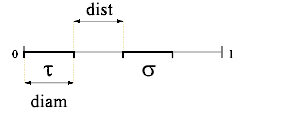
\includegraphics[scale=0.6]{1_2}$$
	$$diam(\tau)\le dist(\tau,\sigma)$$
\end{block}
	
\end{frame}

\begin{frame}
\frametitle{Приклад побудови блочного кластерного дерева}
	\begin{block}{}
		\centering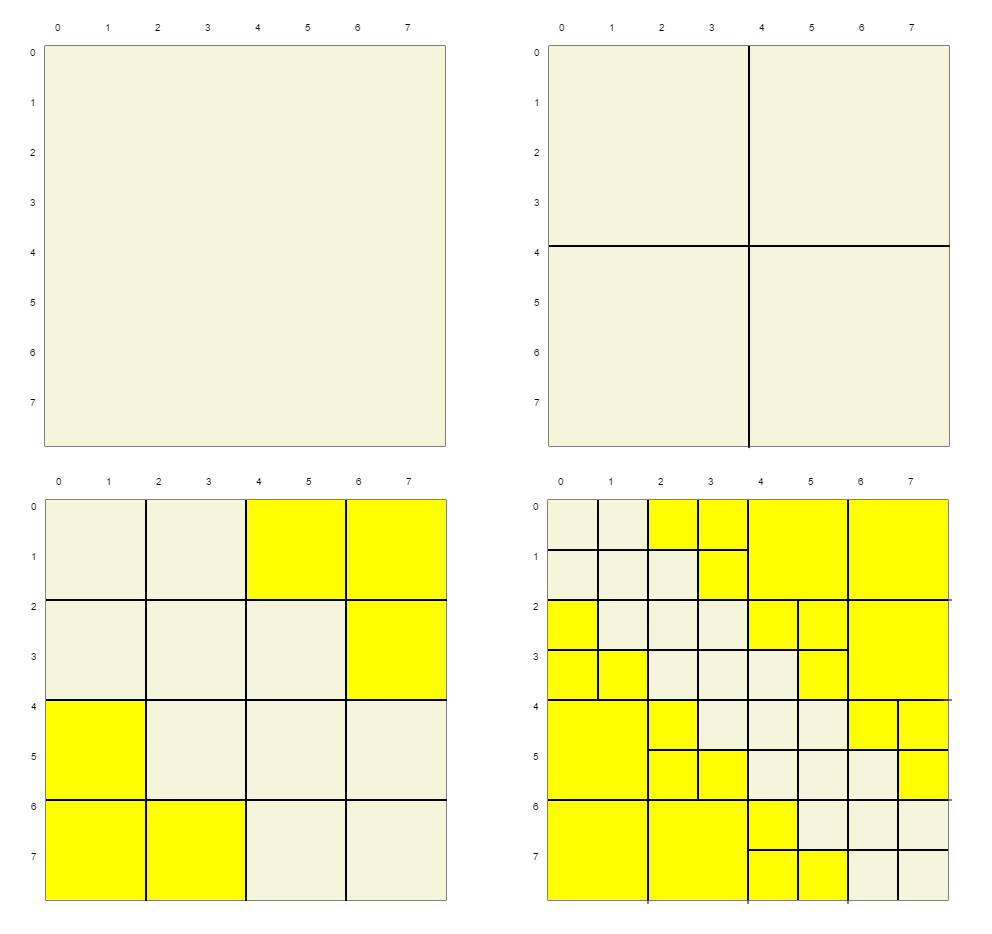
\includegraphics[scale=0.27]{1_3}
	\end{block}
\end{frame}
\begin{frame}
\frametitle{Означення $\mathcal{H}$-матриці}
	\begin{block}{Означення}
		Нехай $\mathbb{T}_{I\times I}$ - блочне кластерне дерево над множиною індексів $I$. Означаємо множину $\mathcal{H}$-матриць як
			$$\mathcal{H}(\mathbb{T}_{I\times I},k):=\{M\in\mathbb{R}^{I\times I}|rank(M|_{t\times s})\le k \text{ для всіх}$$ $$\text{допустимих листків } t\times s \text{ дерева } \mathbb{T}_{I\times I} \}$$
	\end{block}
\end{frame}
\begin{frame}
\frametitle{Метод граничних елементів}
	\begin{block}{}
		Нехай задано функцію $F:[0,1]\rightarrow \mathbb{R}$. Шукаємо функцію $u:[0,1]\rightarrow \mathbb{R}$, яка задовільняє наступне інтегральне рівняння: $$\int_{0}^{1}\ln|x-y|u(y)dy=F(x), x\in[0,1] \eqno(1)$$
	\end{block}
	\begin{block}{Метод Гальоркіна}
	$V_n=span\{\varphi_0,\dots,\varphi_{n-1}\}$
		
		$$\int_{0}^{1}\int_{0}^{1}\varphi_i(x)\ln|x-y|u(y)dydx=\int_{0}^{1}\varphi_i(x)F(x)dx\eqno(2) $$
		
		
	\end{block}
\end{frame}
\begin{frame}{}
	\par Потрібно знайти $u_n$ в просторі $V_n$:
			$$u_n=\sum_{j=0}^{n-1}u_j\varphi_j\eqno(3)$$
			таке, що вектор коефіцієнтів $u$ є розв'язком лінійної системи $$Gu=f$$
			$$G_{ij}=\int_{0}^{1}\int_{0}^{1}\varphi_i(x)\ln|x-y|\varphi_j(y)dydx\eqno(4)$$ 
			$$f_i=\int_{0}^{1}\varphi_i(x)F(x)dx$$
\end{frame}
\begin{frame}
		\begin{block}{}
		Базисні функції визначені як
		\newline 
		\begin{equation*}
		\varphi_i(x)=\begin{cases}
		1,\quad\text{якщо $\frac{i}{n}\le x\le \frac{i+1}{n}$}\\
		0,\quad\text{інакше}
		\end{cases}
		\end{equation*}
	\end{block}
	\begin{block}{}
		Шукаємо наближену матрицю $\tilde{G}$. Для цього заміняємо ядро $g(x,y)=\ln|x-y|$ на розкладене ядро $$\tilde{g}(x,y)=\sum_{v=0}^{k-1}g_v(x)h_v(y)\eqno(5)$$
		Будуємо локальні наближення на підобластях $[0,1]\times[0,1]$, де $g$ є гладкою: $\tau:=[a,b]$, $\sigma:=[c,d]$, $\tau\times\sigma\subset[0,1]\times[0,1]$, $\tau\cap\sigma=\O$.
		
	\end{block}
\end{frame}

\begin{frame}
\frametitle{Геометрична бісекція}
\begin{block}{}
	Ділимо множину індексів $\hat t\in I$, що відповідає кластеру $t$. Для кожного індекса $i \in \hat t$, що відповідає точці $x_i\in\mathbb{R}^n$ можемо визначити
	$$a_l:=\min \{(x_i)_l : i\in \hat t\}$$
	$$b_l:=\max \{(x_i)_l : i\in \hat t\}$$
	для кожного $l\in \{1,...,n\}$. 
	\par Таким чином всі точки знаходяться в паралельній осі коробці $[a_1,b_1]\times...\times[a_n,b_n]$.
\end{block}
\end{frame}
\begin{frame}
\frametitle{Обмежувальні коробки}
\begin{block}{}
Якщо $Q_t=[a_1,b_1]\times...\times[a_n,b_n]$ i $Q_s=[c_1,d_1]\times...\times[c_n,d_n]$, то діаметр і відстань рахуємо за наступними формулами
$$diam(Q_t)=\left(\sum_{l=1}^{n}(b_l-a_l)^2\right)^\frac{1}{2}$$
$$diam(Q_s)=\left(\sum_{l=1}^{n}(d_l-c_l)^2\right)^\frac{1}{2}$$
$$dist(Q_t,Q_s)=\left(\sum_{l=1}^{n}dist([a_l,b_l],[c_l,d_l])^2\right)^\frac{1}{2}$$
\end{block}
\end{frame}
\begin{frame}
\frametitle{Внутрішня задача Діріхле}
\begin{block}{}
Знайти $u\in C^2(\Omega)\cap C(\bar{\Omega}):$
$$\triangle u=0 \text{ в }\Omega$$
$$u=f\text{ на }\Gamma$$
де $f\in C(\Gamma)$ - задана.
\end{block}
\begin{block}{Потенціал простого шару}
$$\Upsilon_{slp}[u](x):=-\frac{1}{2\pi}\int_{\Gamma}\log(|x-y|)u(y)dy$$
\end{block}
\end{frame}
\begin{frame}
\frametitle{Інтерполяція}
\begin{block}{}
Внаслідок інтерпрляції отримуємо
$$\tilde{g}(x,y):=\sum_{v\in K}g(x_v,y)\mathcal{L}_v(x)$$
Відповідні матриці визначені наступним чином
$$A_{iv}:=\int_{\Omega}\varphi_i(x)\mathcal{L}_v(x)dx$$
$$B_{jv}:=\int_{\Omega}\varphi_j(x)\tilde{g}(x_v,y)dy$$
\end{block}
\end{frame}

\begin{frame}
\begin{block}{}
\begin{center}
\Huge{Дякую за увагу!}
\end{center}	
\end{block}
\end{frame}

\end{document}
